\documentclass[a4paper,11pt]{article}

\usepackage[french]{babel}
\usepackage[T1]{fontenc}
\usepackage[utf8x]{inputenc}
\usepackage{lmodern}
\usepackage{microtype}
\usepackage{color}
\usepackage{xcolor}
\usepackage{subcaption}
\usepackage{graphicx}
\usepackage{float}
\usepackage{listings}
\definecolor{olivegreen}{HTML}{3C8031}
\definecolor{commentscolor}{HTML}{777777}
\lstset{
  language=Caml,                % choose the language of the code
  %aboveskip=3mm,
  belowskip=0mm,
  basicstyle={\tt\small},
  numbers=none,                   % where to put the line-numbers
  stepnumber=1,                   % the step between two line-numbers.        
  keywordstyle=\color{blue}, %\textbf,
  stringstyle=\color{olivegreen},
  commentstyle={\itshape\color{commentscolor}},
  numbersep=5pt,                  % how far the line-numbers are from the code
  backgroundcolor=\color{white},  % choose the background color. You must add \usepackage{color}
  showspaces=false,               % show spaces adding particular underscores
  showstringspaces=false,         % underline spaces within strings
  showtabs=false,                 % show tabs within strings adding particular underscores
  tabsize=2,                      % sets default tabsize to 2 spaces
  captionpos=b,                   % sets the caption-position to bottom
  breaklines=true,                % sets automatic line breaking
  breakatwhitespace=true,         % sets if automatic breaks should only happen at whitespace
  title=\lstname,                 % show the filename of files included with \lstinputlisting;
  escapeinside={</}{/>},
}

\usepackage{hyperref}

\newcommand{\caml}[1]{\lstinline{#1}}
\newcommand{\question}[2][]{
  \subsection*{Question #2 : \tt{#1}}
  \addcontentsline{toc}{subsection}{Question #2 : \tt{#1}}
}
\newcommand{\comment}[1]{}

\title{Rapport de projet\\Programmation fonctionnelle}
\author{Lilian MALLARDEAU}
\date{Semestre 2}

\begin{document}

\maketitle
\tableofcontents
\pagebreak

% ------------ Préambule ------------ %
\section*{Préambule}
\addcontentsline{toc}{section}{Préambule}
Le sujet du projet portait sur les formules de la logique propositionnelle. Une formule logique (ou proposision) est une affirmation qui peut être vraie ou fausse : on lui associe donc sa valeur de vérité, \textit{V} (vrai) ou \textit{F} (faux).

Les proposisions sont formées avec des variables logiques (qui peuvent également être vraies ou fausses), et des connecteurs (ou $\lor$, et $\land$, \dots).

\bigskip

On s'intéresse plus particulièrement dans le sujet à une représentation des tables de vérités des formules logiques par des arbres. D'abord, on représente la formule par un arbre binaire, dans lequel chaque nœud correspond à une variable et chaque sous arbre (respectivement de droite ou de gauche) correspond au sous arbre de décision de la formule en remplaçant la variable du nœud par vrai ou faux.

\bigskip

Ensuite, on s'intéresse au \textit{Binary Decision Diagram}, l'idée étant de simplifier notre arbre de décision, d'abord en repérant les redondances et en les éliminant, puis en simplifiant les nœuds qui ont le même successeur.

\bigskip

Enfin, on utilisera Dot pour générer des graphiques de nos arbres.


\pagebreak

% ------------ Arbres de décision ------------ %
\section*{Arbres de décision}
\addcontentsline{toc}{section}{Arbres de décision}

Afin de pouvoir manipuler aisément les formules logiques en Caml, on définit tout d'abord un type \caml{tformula} :

\begin{lstlisting}
  type tformula =
  | Value of bool (* </$\bot$/> ou </$\top$/> *)
  | Var of string (* Variable *)
  | Not of tformula (* Negation *)
  | And of tformula * tformula (* Conjonction *)
  | Or of tformula * tformula (* Disjonction *)
  | Implies of tformula * tformula (* Implication *)
  | Equivalent of tformula * tformula (* Equivalence *)
\end{lstlisting}

Ainsi, une formule est soit une valeur de vérité (vrai ou faux) ou une variable, soit une composée d'autres formules et opérateurs ($\land$, $\lor$, $\neg$, \dots).

\bigskip

On définit également un type \caml{decTree} pour représenter un abre de décision, en consirérant qu'un arbre est soit une feuille (vrai ou faux), soit un nœud qui possède un nom (le nom de la variable correspondant au nœud) et ses deux sous arbres \comment{(respectivement de gauche et de droite)}:

\begin{lstlisting}
  type decTree =
  | DecLeaf of bool
  | DecRoot of string * decTree * decTree
\end{lstlisting}

\question[getVars : tformula -> string list]{1}
La première question consiste à écrire une fonction \caml{getVars}, qui sur la donnée d'une formule nous renvoit la liste des variables présentes dans la formule, triée par ordre croissant et sans doublon.

Il a suffit pour cela de définir une fonction auxiliaire récursive, 
puis d'appliquer \caml{List.sort_uniq compare} pour trier la liste en s'assurant que chaque élément n'y apparaisse qu'une fois (\caml{compare} étant l'ordre naturel sur les chaînes de caractères).

\question[evalFormula : env -> tformula -> bool]{2}
Afin de pouvoir évaluer une formule, on doit connaître la valeur des variables apparaissant dans la formule : on définit pour cela un \textbf{environnement} comment étant une liste de couples \caml{(nom_variable, valeur)} :

\begin{lstlisting}
  type env = (string*bool) list
\end{lstlisting}

On peut maintenant définir une fonction récursive \caml{evalFormula}, qui prend en paramètres une formule et un environnement, et qui évalue cette formule dans cet environnement.

Pour cela, j'ai défini une fonction \caml{getVarValue : env -> string -> bool}, qui prend en paramètres un environnement et le nom d'une variable, et renvoit la valeur de la variable dans l'environnement.

La fonction \caml{evalFormula} se réduit donc à un pattern matching sur la formule, en appliquant les règles de logique pour déterminer la valeur de vérité de la formule en fonction des opérateurs, et en appelant la fonction \caml{getVarValue} lorsqu'une formule est de type \caml{Var(_)}.

\question[buildDecTree : tformula -> decTree]{3}
On définit la fonction \caml{buildDecTree : tformula -> decTree} qui construit l’arbre de décision d’une formule.

Pour construire l'arbre de décision, on doit construire l'environnement au fur et à mesure de la construction de l'arbre : pour cela, j'ai défini une fonction auxiliaire, qui prend l'environnement en tant qu'accumulateur, et la liste des variables qui n'ont pas encore été ajoutées à l'environnement. Lorsque toutes les variables ont été ajoutées à l'environnement, on peut évaluer la formule (et renvoyer un \caml{DecLeaf}), sinon on fait deux appels récursifs, en ajoutant respectivement la valeur \caml{true} et \caml{false} pour la variable actuelle dans l'environnement :

\begin{lstlisting}
  let rec aux formula env vars = match vars with
    | [] -> DecLeaf (evalFormula env formula)
    | h::t -> DecRoot(h, aux formula ((h,true)::env) t, aux formula ((h,false)::env) t)
\end{lstlisting}

Il faut ensuite appeler la fonction auxiliaire avec un accumulateur vide et la liste des variables présentes dans la formule :

\begin{lstlisting}
  aux formula [] (getVars formula);;
\end{lstlisting}


% ------------ Binary Decision Diagram ------------ %
\section*{Binary Decision Diagram}
\addcontentsline{toc}{section}{Binary Decision Diagram}

On cherche maintenant non plus à constuire un arbre, mais un graphe (\textit{Binary Decision Diagram}), dont le chemin choisi définit les valeurs de chaque variable, et l'extrémité du chemin la valeur de la formule calculée avec l'environnement défini par le chemin. On représente un tel graphe par une liste de nœuds \caml{bddNode}, chacun ayant un numéro, et dans le cas d'une feuille, sa valeur (\caml{false} ou \caml{true}), ou dans le cas d'un nœud, le nom de la variable auquel il correspond et les numéros de ses deux sous nœuds (correspondants aux deux valeurs possibles de la variable) :

\begin{lstlisting}
  type bddNode =
  | BddLeaf of int * bool
  | BddNode of int * string * int * int;;
\end{lstlisting}

Le BDD quant à lui est la donnée de la liste des nœuds définis précédement et du numéro du nœud racine :
\begin{lstlisting}
  type bdd = (int * (bddNode list));;
\end{lstlisting}
  
\question[buildBdd : tformula -> bdd]{4}
La fonction \caml{buildBdd} construit le BDD d'une formule. Pour cela, il faut vérifier à chaque étape de la construction du graphe que le nœud qu'on s'apprête à construire n'est pas déjà présent dans la liste. Si ce n'est pas le cas, on l'ajoute à la liste avec un nouveau numéro. Si c'est le cas, on référence à la place le nœud déjà existant.

Par soucis de simplicité et de clareté, j'ai choisi de définir d'abord deux fonctions :
\begin{itemize}
  \item la fonction \caml{getBddNodeId : bddNode list -> bddNode -> int}, qui nous donne le numéro d'un nœud dans la liste s'il y est présent, et -1 sinon
  \item la fonction \caml{getMaxNodeId : bddNode list -> int} qui nous renvoie le plus grand numéro attribué à un nœud dans la liste (pour pouvoir assigner un numéro à un nouveau nœud plus facilement)
\end{itemize}

\bigskip

Comme pour la fonction \caml{buildDecTree}, la fonction \caml{buildBdd} doit construire l'environnement au fur et à mesure des appels récursifs ; il est donc nécessaire, de même que pour la fonction \caml{buildDecTree}, d'avoir un accumulateur pour l'environnement d'évaluation de la formule.

De plus la fonction \caml{buildBdd} doit renvoyer un \caml{bdd}, c'est-à-dire un couple \caml{(int * bddNode list)}, j'ai donc défini une fonction auxiliaire récursive \caml{aux}, qui prend en paramètres \caml{bddNodeList} la liste des nœuds déjà créés, \caml{formula} la formule, \caml{env} l'accumulateur pour l'environnement et \caml{vars} la liste des variables qui n'ont pas encore été ajoutées à l'environnement, et qui renvoit un \underline{\underline{\caml{bdd}}} (donc un couple \caml{(int * bddNode list)}), et non pas seulement la liste des nœuds :

\begin{lstlisting}
  let rec aux bddNodeList formula env vars
  (* aux : bddNode list -> tformula -> env -> string list -> bdd *)
\end{lstlisting}

Pour déterminer si on doit créer un \caml{BddNode} ou un \caml{BddLeaf}, \caml{aux} fait un pattern matching sur \caml{vars} :
\begin{itemize}
  \item si \caml{vars = []}, alors tout l'environnement a été construit et donc toutes les variables se trouvent dans \caml{env}. On crée alors un \caml{BddLeaf} en déterminant son numéro avec \caml{getMaxNodeId}, et on vérifie qu'il n'existe pas déjà dans le bdd avec \caml{getBddNodeId}. Si il n'existe pas encore, on renvoit le couple \caml{(m, node::bddNodeList)}, pour ajouter le nœud \caml{node} nouvellement créé à la liste des nœuds (\caml{m} étant le numéro du nouveau nœud). Sinon, on renvoit \caml{(n, bddNodeList)}, \caml{n} étant le numéro du nœud existant (on n'ajoute donc pas le nœud \caml{node} à la liste).
  \item Si \caml{vars} n'est pas vide (\caml{vars = h::t}), on doit créer un \caml{BddNode} avec les deux sous-nœuds correspondants. On fait deux appels récursifs à \caml{aux} en récupérant la liste des nœuds mise à jour et les numéros des deux nœuds suivants, on crée notre nouveau nœud avec les numéros de ses successeurs, et on renvoit (de même que pour le cas précédent) la liste des nœuds augmentée du nœud actuel avec son numéro s'il n'est pas déjà présent dans la liste (donc \caml{(m, node::bddNodeList)}), et le numéro du nœud déjà existant avec la liste actuelle sinon.
\end{itemize}

Il suffit ensuite d'appeler la fonction auxiliaire avec une liste de nœuds vide et un environnement vide pour obtenir le BDD complet :
\begin{lstlisting}
  aux [] formula [] (getVars formula);;
\end{lstlisting}


% ------------ BDD simplifié ------------ %
\section*{BDD simplifié}
\addcontentsline{toc}{section}{BDD simplifié}
\question[simplifyBDD : bdd -> bdd]{5}

L'objectif est maintenant de simplifier le graphe en supprimant les nœuds qui ont deux fois le même successeur. On définit pour cela la fonction \caml{simplifyBDD : bdd -> bdd}.

Encore par soucis de simplicité, j'ai défini une fonction \caml{simplifyNode : bddNode list -> int -> int -> bddNode list}, qui prend la liste des nœuds du graphe, deux entier \caml{n} et \caml{p}, et qui renvoit la liste modifiée, en ayant supprimé le nœud \caml{BddNode(n, _, p, p)} et modifié les nœuds pointant vers \caml{n} pour qu'ils pointent vers \caml{p}.

\medskip

La fonction \caml{simplifyBDD} doit alors parcourir la liste des nœuds du graphe, et appeler la fonction \caml{simplifyNode} pour chaque nœud de la forme \caml{BddNode(_, _, p, p)}.

Bien que cela puisse paraître simple à première vue, c'est en fait plus délicat qu'on peut le penser. J'ai d'abord cherché des moyens de parcourir une liste en la modifiant en même temps, ce qui est compliqué puisqu'on n'a pas seulement besoin de modifier l'élément courant lors du parcours, mais également tous les autres nœuds qui le référencent.

La solution que j'ai trouvé a été de définir une fonction auxiliaire qui prend en argument le bdd à simplifier (qu'elle va mettre à jour à chaque appel récursif), mais également la liste des nœuds présents initialement dans celui-ci :
\begin{lstlisting}
  let rec aux (bdd : bdd) (bddNodeList : bddNode list)
\end{lstlisting}

Ainsi, on peut lors des appels récursifs parcourir la liste des nœuds \caml{bddNodeList}, en vérifiant pour chaque nœud s'il peut être supprimé du graphe, et mettre à jour le bdd complet lorsque nécessaire à l'aide de \caml{simplifyNode}.

Il faut également penser à mettre à jour le numéro du nœud racine du BDD, si jamais celui-ci peut être simplifié.

\smallskip

Après avoir défini la fonction \caml{aux} ainsi, il ne reste plus qu'à faire un pattern matching sur le bdd reçu en paramètre, pour faire l'appel initial en envoyant une "copie" de la liste des nœuds du bdd :
\begin{lstlisting}
  match bdd with
    | (m, l) -> aux bdd l;;
\end{lstlisting}


% ------------ Vérification de formules ------------ %
\section*{Vérification de formules}
\addcontentsline{toc}{section}{Vérification de formules}

\question[isTautology : tformula -> bool]{6}
Avec la simplification de la question précédente, toute tautologie se réduit à un seul nœud : la feuille true. On peut donc définir aisément une fonction \caml{isTautology : tformula -> bool} qui vérifie si une formule est une tautologie :
\begin{lstlisting}
  let isTautology (formula : tformula) =
    (simplifyBDD (buildBdd formula)) = (1, [BddLeaf (1, true)]);;
\end{lstlisting}

\question[areEquivalent : tformula -> tformula -> bool]{7}
On souhaite faire une fonction \caml{areEquivalent}, qui teste si deux formules sont équivalentes.
On peut simplement utiliser la fonction précédente :
\begin{lstlisting}
  let areEquivalent (formula1 : tformula) (formula2 : tformula) =
    isTautology (Equivalent(formula1, formula2));;
\end{lstlisting}


% ------------ Affichage graphique de BDD ------------ %
\section*{Affichage graphique de BDD}
\addcontentsline{toc}{section}{Affichage graphique de BDD}

On utilise DOT pour générer graphiquement les arbres et BDD des formules. Il faut cependant générer le fichier .dot contenant la description du graphe. On définit pour cela deux fonctions :

\question[dotBDD : string -> bdd -> unit]{8}
On créé une fonction \caml{dotBDD : string -> bdd -> unit} qui prend un nom de fichier et un bdd et qui génère le fichier Dot correspondant.

Dans le fichier .dot, on doit identifier chaque nœud avec un numéro pour que DOT puisse faire le lien entre chaque nœud ; ce qui est plutot pratique dans le cas d'un BDD, puisque chaque nœud possède déjà un numéro.

J'ai donc défini une fonction auxiliaire récursive qui prend la liste des nœuds, et qui imprime dans le fichier les lignes correspondantes. Cette fonction fait un pattern matching sur le type du nœud, (\caml{BddNode} ou \caml{BddLeaf}), et imprime à l'aide de \caml{fprintf} les lignes nécessaires pour faire apparaître dans le graphe le nœud et les deux arcs le reliant aux suivants. Par exemple,
\begin{lstlisting}
  fprintf file "%d [style = bold, label=\"%B\"];\n" id value;
\end{lstlisting}
permet d'afficher la feuille de numéro \caml{id} et ayant comme valeur \caml{value}.
On fait ensuite un appel récursif sur la suite de la liste.

Il faut cependant imprimer au début du fichier l'instruction DOT pour commencer le graphe, et une accolade à la fin pour indiquer la fin du graphe. On utilise de même \caml{fprintf} pour imprimer ces lignes, en appelant la fonction auxiliaire sur la liste complète entre les deux :
\begin{lstlisting}
  fprintf file "digraph G {\n";
  match bdd with
    | (m, l) -> aux file l;
  fprintf file "}";
\end{lstlisting}

\question[dotDec: string -> decTree -> unit]{9}

Ici, on cherche à générer le fichier .dot, mais on part d'un arbre binaire. Le principe est le même, cependant cette fois ci les nœuds ne sont pas numérotés dans le \caml{decTree} : il va falloir leur associer un numéro unique au fur et à mesure du parcours de l'arbre.

Après une certaine réflexion, j'ai eu l'idée, pour numéroter les successeurs d'un nœud de façon unique, d'ajouter respectivement $1$ et $2$ à la fin de la chaine de caractère du numéro du nœud parent : cela revient, pour un nœud $n$, à numéroter ses successeurs $10n+1$ et $10n+2$. On aurait ainsi la numérotation suivante :
\begin{figure}[H]
  \centering
  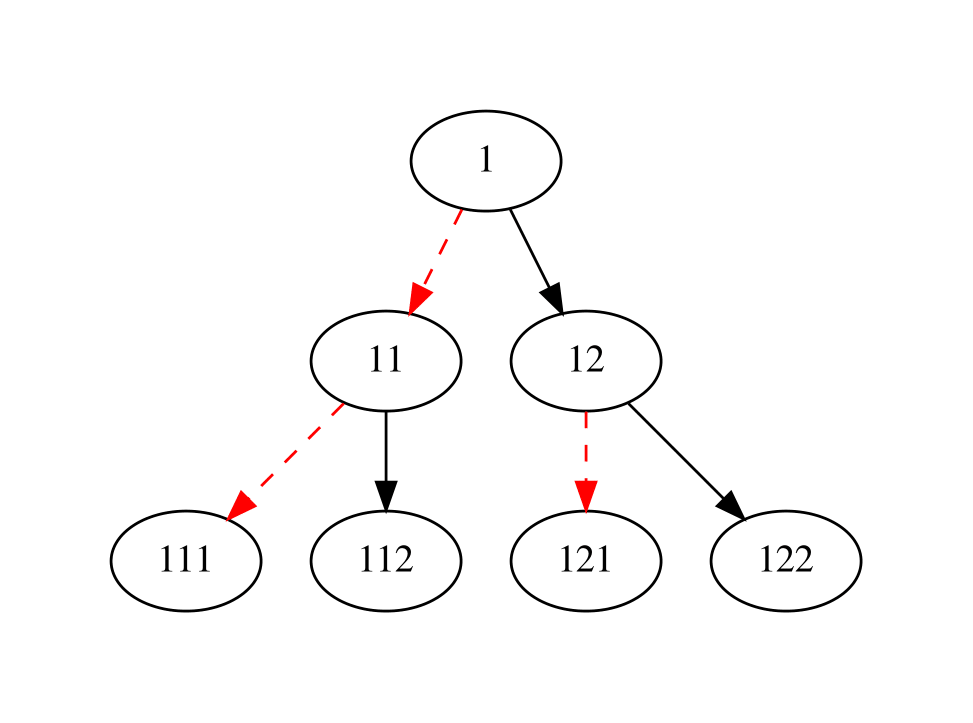
\includegraphics[scale=0.25]{binary_numerotation.png}
\end{figure}

La fonction \caml{dotDec} est semblable à la fonction \caml{dotBdd} précédente. On adapte seulement la fonction auxiliaire pour qu'elle prenne en plus un entier $n$, numéro du nœud à ajouter au fichier, et on fait les appels récursifs sur les nœuds successeurs avec respectivement $10n+1$ et $10n+2$ comme numéro.

Pour l'appel initial, on envoit la racine de l'arbre complet, numéroté 1 :
\begin{lstlisting}
  fprintf file "digraph G {\n";
  aux file 1 tree;
  fprintf file "}";
\end{lstlisting}

\medskip

De façon plus intelligente, on aurait pu aussi remarquer qu'en assignant le numéro 1 au premier nœud et en attribuant les numéros $2n+1$ et $2n+2$ aux successeurs d'un nœud $n$, on obtient la même numérotation que si on avait attribué les numéros à chaque nœud un par un, de haut en bas et de gauche à droite.

\bigskip
\bigskip

\section*{Note}
J'ai aidé certains de mes camarades pour certaines questions, en particulier pour les questions 4 et 5. Il est donc possible que quelques étudiants aient un code similaire au mien, en particulier pour ces questions.


% ------------ Annexes : tests ------------ %
\pagebreak
\section*{Annexes : tests}
\addcontentsline{toc}{section}{Annexes : tests}

\subsection*{$A \Rightarrow B \Leftrightarrow B \lor \lnot A$}
\addcontentsline{toc}{subsection}{$A \Rightarrow B \Leftrightarrow B \lor \lnot A$}
\begin{figure}[!htb]
  \begin{minipage}{0.5\textwidth}
    \centering
    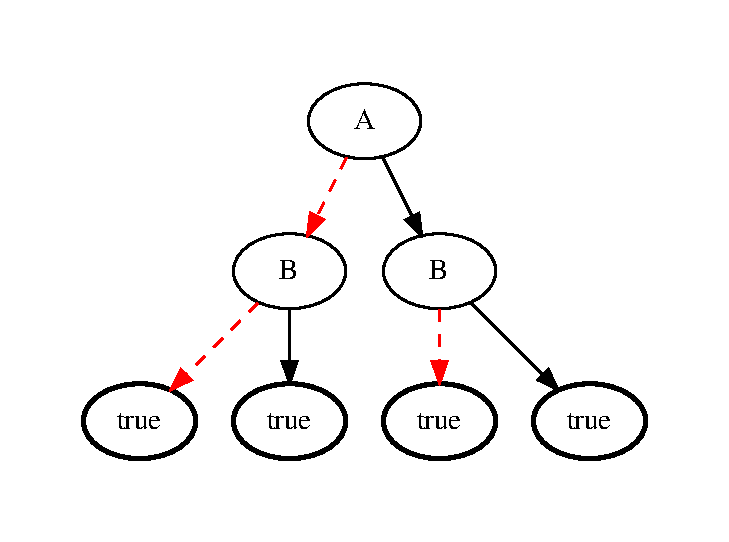
\includegraphics[width=1\linewidth]{tests_rapport/test2_dectree.pdf}
    \caption*{Arbre de décision}
  \end{minipage}\hfill
  \begin{minipage}{0.25\textwidth}
    \centering
    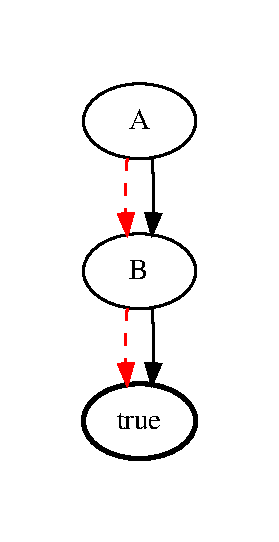
\includegraphics[width=1\linewidth]{tests_rapport/test2_bdd.pdf}
    \caption*{BDD}
  \end{minipage}\hfill
  \begin{minipage}{0.24\textwidth}
    \centering
    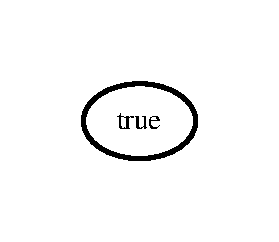
\includegraphics[width=1\linewidth]{tests_rapport/test2_simplified_bdd.pdf}
    \caption*{BDD simplifié}
  \end{minipage}
\end{figure}

\subsection*{$(Q_1 \Leftrightarrow Q_2) \lor (P_1 \Leftrightarrow P_2)$}
\addcontentsline{toc}{subsection}{$(Q_1 \Leftrightarrow Q_2) \lor (P_1 \Leftrightarrow P_2)$}
\begin{figure}[!htb]
  \begin{minipage}{1\textwidth}
    \centering
    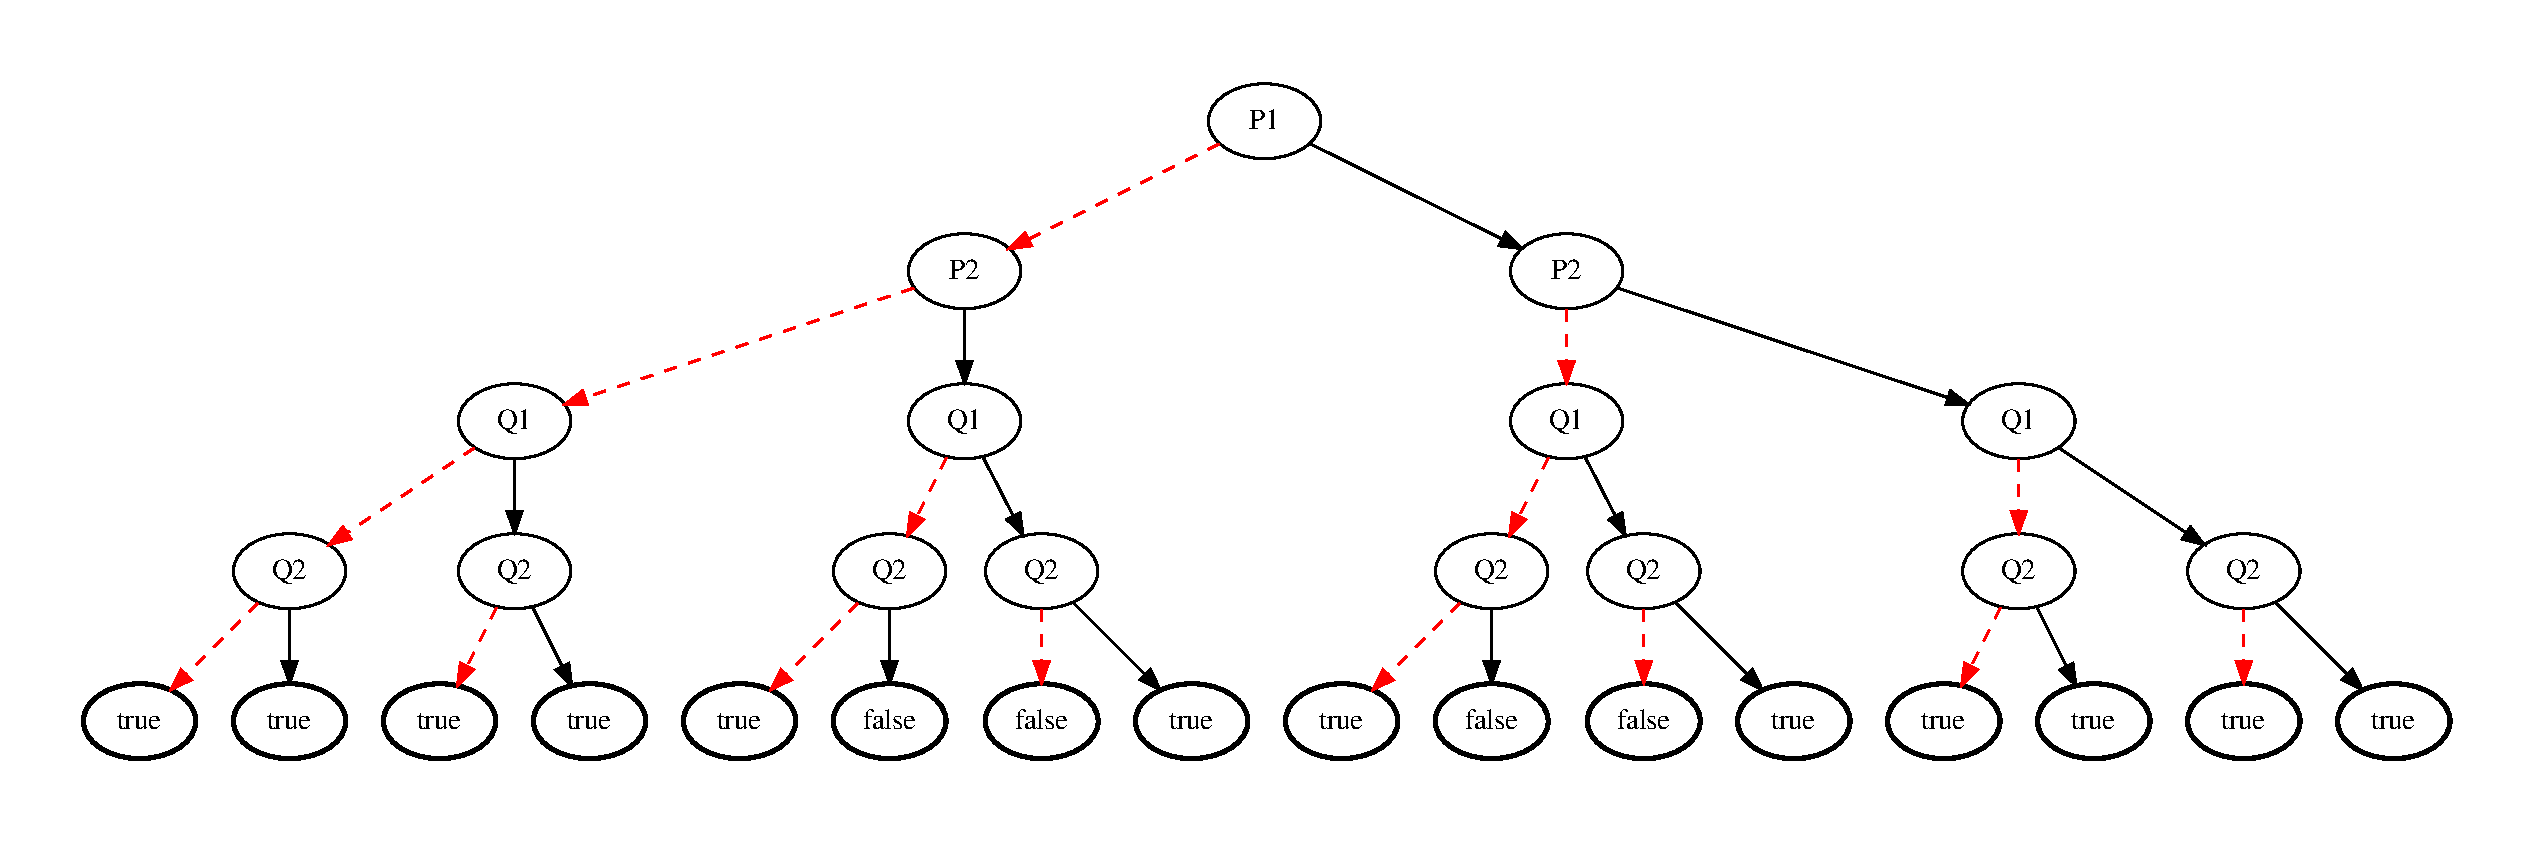
\includegraphics[width=0.8\linewidth]{tests_rapport/test1_dectree.pdf}
    \caption*{Arbre de décision}
  \end{minipage}
  \begin{minipage}{0.25\textwidth}
    \centering
    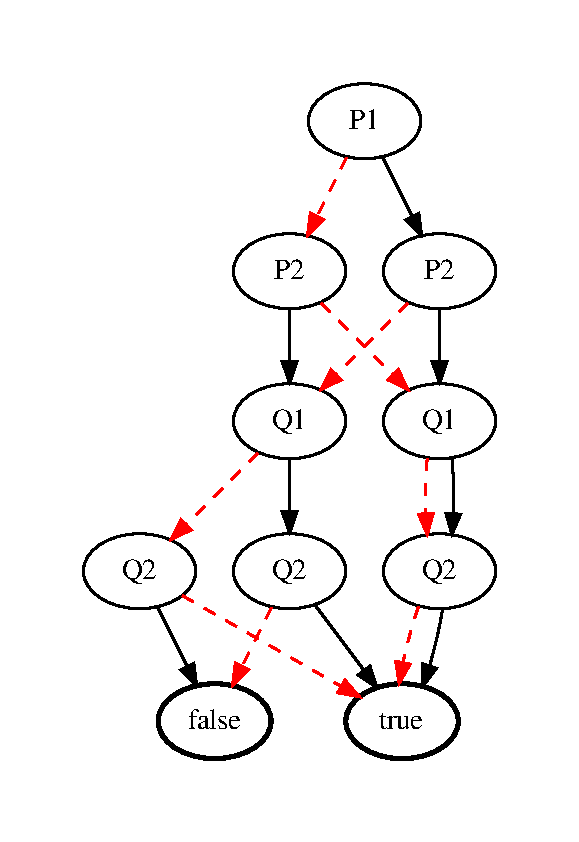
\includegraphics[width=0.8\linewidth]{tests_rapport/test1_bdd.pdf}
    \caption*{BDD}
  \end{minipage}\hfill
  \begin{minipage}{0.25\textwidth}
    \centering
    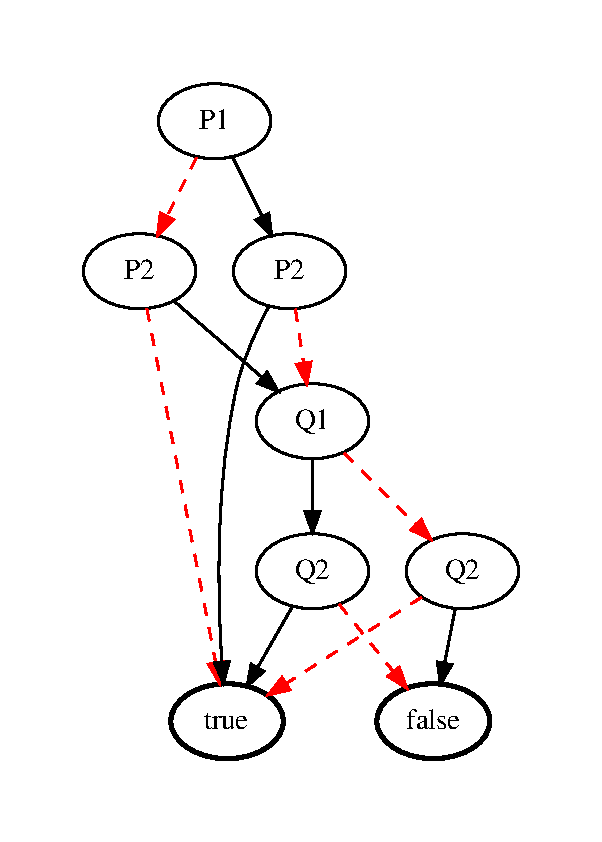
\includegraphics[width=0.8\linewidth]{tests_rapport/test1_simplified_bdd.pdf}
    \caption*{BDD simplifié}
  \end{minipage}
\end{figure}


\end{document}